\documentclass[letterpaper,12pt]{article}
\usepackage[spanish]{babel}
\spanishdecimal{.}
\usepackage[utf8]{inputenc}
\usepackage{graphicx}
\usepackage[top=2.5cm, bottom=2.5cm, left=2.5cm, right=2.5cm]{geometry}
\usepackage{hyperref}

\title{Práctica 2 \\ Instalación de Software para Operar Robots Bípedos}
\author{Robots Bípedos Autónomos}
\date{Facultad de Ingeniería, UNAM}


\begin{document}
\renewcommand{\tablename}{Tabla}
\maketitle
\section*{Objetivos}
\begin{itemize}
\item Familiarizar al alumno con el uso del software de control de versiones \texttt{git}.
\item Aprender a utilizar el software desarrollado para la operación de robots bípedos autónomos.
\item Familiarizar al estudiante con el simulador Gazebo.
\end{itemize}

\section{Introducción}
\textbf{Git.} Es un software de control de versiones \textit{open source}, creado por Linus Torvalds. Está pensado para el desarrollo de software cuando éste posee una gran cantidad de código fuente y facilita el trabajo cooperativo mediante el manejo de \textit{branching} y herramientas de solución de conflictos. 

En este curso se usará \texttt{git} para el manejo de versiones del software necesario para operar el robot que se utilizará en el desarrollo de prácticas y proyectos. Además, proporcionará al alumno herramientas para desarrollar de forma ordenada todos los códigos necesarios.

En la página \url{https://git-scm.com/} se pueden encontrar tutoriales para aprender más sobre \texttt{git}.

\section{Desarrollo}
\subsection{Instalación de Git y obtención del software}
\textbf{Nota.} Se asume que el alumno ya tiene instalado Ubuntu 16.04 y ROS kinetic. 

En una terminal, teclear los siguientes comandos:
\begin{verbatim}
$  sudo apt-get install git
$  cd
$  git clone https://github.com/mnegretev/PAPIME_PE116219
$  cd PAPIME_PE116219
\end{verbatim}
Lo anterior descarga una copia del repositorio que contiene el material a usar durante el curso. Para descargar una actualización, teclee el siguiente comando:
\begin{verbatim}
$  git pull origin master
\end{verbatim}
Puesto que en este momento no hay ninguna actualización disponible, se debe leer la siguiente salida:
\begin{verbatim}
From https://github.com/mnegretev/RoboticsCourses
 * branch            master    -> FETCH_HEAD
Already up-to-date.
\end{verbatim}

\subsection{Instalación de dependencias y compilación}
Para poder compilar y ejecutar el software, es necesario instalar varias dependencias. Para ello, en una terminal teclee los siguientes comandos:
\begin{verbatim}
    $  cd
    $  cd PAPIME_PE116219/SoftwareHumanoide
    $  sudo ./Setup.sh
\end{verbatim}

Esto comenzará a instalar varias bibliotecas y algunos paquetes de ROS necesarios. Cuando el script termine de ejecutarse, teclee los siguientes comandos para compilar el código:
\begin{verbatim}
    $  cd
    $  cd PAPIME_PE116219/SoftwareHumanoide
    $  catkin_make -j2 -l2
\end{verbatim}

Una vez finalizada la compilación, ejecute los siguientes comandos:

\begin{verbatim}
    $  cd  ~/PAPIME_PE116219/SoftwareHumanoide
    $  source devel/setup.bash
    $  export GAZEBO_MODEL_PATH=~/PAPIME_PE116219/SoftwareHumanoide/src
          /hardware/nimbro_op_gazebo/models/:${GAZEBO_MODEL_PATH}
    $  roslaunch surge_et_ambula humanoid_simul.launch
\end{verbatim}

Se mostrará una ventana como la que se observa en la figura \ref{fig:gazebo}. Presione el botón que se muestra encerrado en un cuadro rojo en la misma figura. Aparecerán otras dos ventanas como las que se muestran en las figuras \ref{fig:gui} y \ref{fig:rviz}.

En otra terminal, ejecute el comando y observe lo que sucede en el simuador Gazebo y en el visualizador RViz. 
\begin{verbatim}
    $  rostopic pub /hardware/head_goal_pose std_msgs/Float32MultiArray 
          "{data:[0, 0.2]}"
\end{verbatim}

El comando anterior \textit{publica} el \textit{tópico} \texttt{/hardware/head\_goal\_pose}, que acepta \textit{mensajes} de tipo \texttt{Float32MultiArray}. El valor publicado es un arreglo de dos flotantes $[0.0, 0.2]$. El \textit{nodo} \texttt{/hardware/control\_remapper} está \textit{suscrito} a este tópico y lo que hace es mover la cabeza del robot a un par de ángulos pan-tilt. El movimiento tilt positivo es hacia abajo para seguir la convención de la mano derecha en el sistema de referencia de la cabeza. 

\begin{figure}
\centering
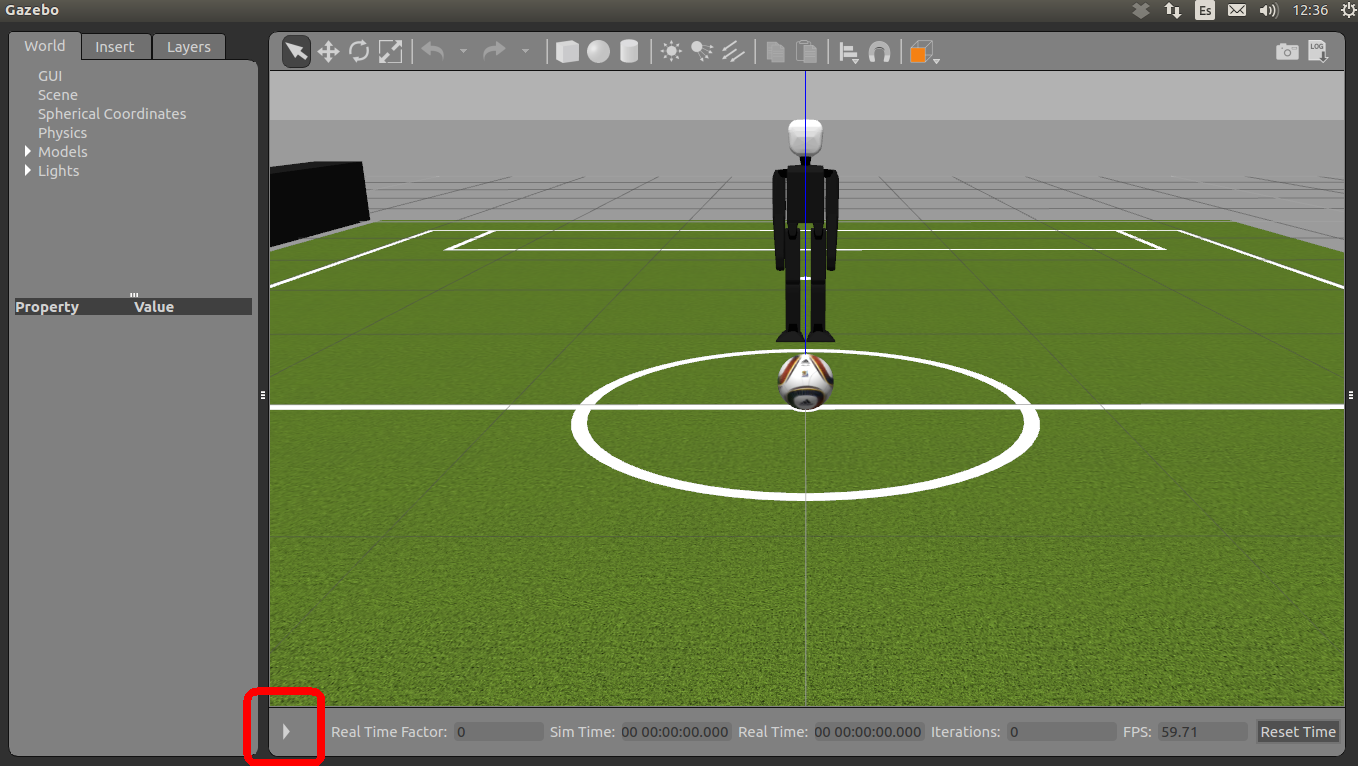
\includegraphics[width=0.9\textwidth]{gazebo_initial.png}
\caption{El simulador Gazebo.}
\label{fig:gazebo}
\end{figure}

\begin{figure}
\centering
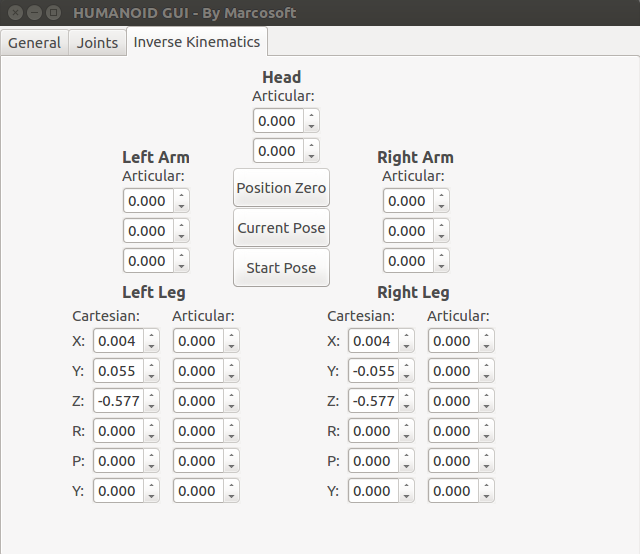
\includegraphics[width=0.6\textwidth]{gui.png}
\caption{Interfaz gráfica para operación del robot bípedo.}
\label{fig:gui}
\end{figure}

\begin{figure}
\centering
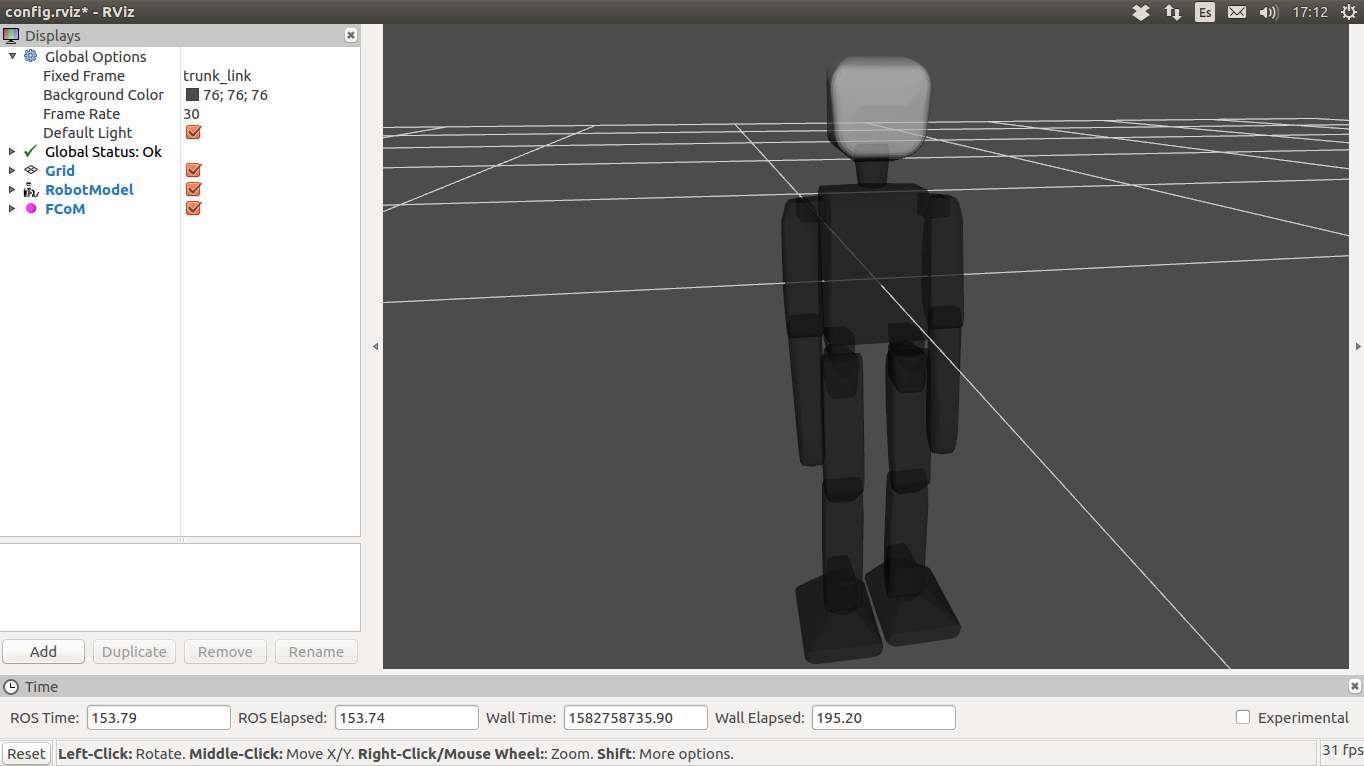
\includegraphics[width=0.9\textwidth]{rviz.png}
\caption{El visualizador RViz.}
\label{fig:rviz}
\end{figure}

\subsection{Nodo para mover la cabeza del robot}
Escriba un nodo que publique en el tópico \texttt{/hardware/head\_goal\_pose} los ángulos pan-tilt necesarios para que la cabeza del robot describa un gesto de ``sí'', es decir, que mueva la cabeza de arriba a abajo. El tópico debe publicarse 10 veces por segundo. El lenguaje puede ser C++ o Python.

\section{Evaluación}
Para que la práctica se considere entregada se deben cumplir los siguientes puntos:
\begin{itemize}
\item El movimiento del robot en el visualizador debe describir claramente el gesto ``sí''.
\item El comando \texttt{rostopic echo} debe mostrar que el tópico se está publicando correctamente.
\end{itemize}

\end{document}
%%% Local Variables:
%%% mode: latex
%%% TeX-master: t
%%% End:
